\chapter{Besaid}

\begin{enumerate}
	\item \cs[0:30], \sd, \fmv. Swim to the beach and \sd. Walk up to \wakka, \sd, walk down to next screen.
	\item Walk right to next screen, right again, down to \wakka.
	\item Swim in the Lagoon. Watch out for invisible wall at the end.
\end{enumerate}
\begin{encounters}
	\begin{itemize}
		\item Piranhas:
		      \begin{itemize}
			      \item Attack if 2 groups, or 3 if preempt.
			      \item Otherwise run away.
		      \end{itemize}
	\end{itemize}
\end{encounters}
\begin{enumerate}[resume]
	\item \sd\ next couple of screens. Walk to temple, \cs[0:30]. Walk to the Priest, \cs[1:30]. Walk to \wakka\ tent (middle right), talk to him and \sd
	\item Walk to temple, \sd
\end{enumerate}
\begin{trial}
	\begin{itemize}
		\item Touch the wall at the end
		\item Touch the wall on the right
		\item Go down the steps and pickup the sphere from the wall
		\item Go down the steps and place the sphere in the door
		\item Go down the corridor past the first pedestal
		\item Touch the wall opposite the second pedestal to open the hidden room
		\item Pickup the sphere in the hidden room, place it on the second pedestal
		\item Push the pedestal to complete the trials
	\end{itemize}
\end{trial}
\begin{enumerate}[resume]
	\item \cs[1:00], \sd\ inside the Fayth room. \fmv+\cs[1:00]. \sd\ after the \fmv, walk down to Besaid Center. \cs[1:40], name \valefor.
	\item \sd\ at party, walk to \yuna. \sd, respond with the \nth{2} option, ``She's not my type''. Talk to \wakka, go to sleep, \sd\ on the dream docks.
	\item Walk out of tent, \sd.
	\item Go back to Besaid, talk to the shop owner in the bottom left tent. Talk to the dog in the top right tent.
	\item Leave village, \sd\ through forced encounters, \sd\ during cutscene, avoid statue and leave the area by going up. You get 2 Power Spheres from these tutorials. \skippablefmv\ right before the \kimahri\ fight.
\end{enumerate}
\begin{spheregrid}
	\begin{itemize}
		\item \textit{If \tidus\ has 3 levels:}
		      \begin{itemize}
			      \item Move $\leftarrow$
			      \item Get Cheer, Str +1
		      \end{itemize}
		      \ifthenelse{\equal{\colstyle}{multi}}{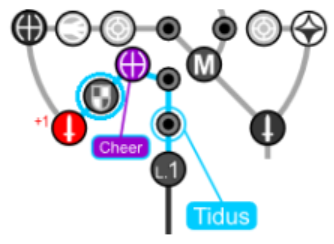
\includegraphics[width=.7\columnwidth]{graphics/tiduscheer}}{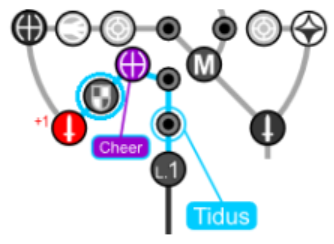
\includegraphics[width=.4\columnwidth]{graphics/tiduscheer}}
	\end{itemize}
\end{spheregrid}
\begin{battle}[750]{Kimahri}
	\begin{itemize}
		\tidusf Attack x3-7, depending on crits/Strength node.
		\tidusf Each attack does average of 125, so 6 attacks averaging that will kill.
		\tidusf Need either Str Node, 2 Evades, 1 Crit, or +7 damage, otherwise Potion after 5th \tidus' Attack
	\end{itemize}
\end{battle}
\begin{enumerate}[resume]
	\item \sd, continue running
\end{enumerate}
\begin{battle}{Garuda}
	\begin{itemize}
		\summon{\valefor}
		\valeforf Thunder x6 to build \od
	\end{itemize}
Guaranteed 1 Power Sphere.
\end{battle}
\begin{enumerate}[resume]
	\item If you didn't do the sphere grid yet, do it now.
	\item \formation{\tidus}{\yuna}{\lulu}
\end{enumerate}
\begin{battle}{Garuda}
	\begin{itemize}
		\item Flee using the Escape Command
	\end{itemize}
\end{battle}
\begin{encounters}
	\begin{itemize}
		\item Dingo: \tidus\ Attack
		\item Condor: \wakka\ Attack
		\item Water Flan: \lulu\ Thunder
	\end{itemize}
\end{encounters}
\begin{enumerate}[resume]
	\item At Besaid Beach go onto the boat.
\end{enumerate}